\section{Backup Slides}

\begin{frame}{}
 \begin{alertblock}{}
  \centering
  \huge{
  Backup slides
  }
 \end{alertblock}
\end{frame}
	
\begin{frame}
\frametitle{Observatorio Pierre Auger (PAO)}
\framesubtitle{Descripci\'on}
	\begin{block}{Detector - Tama\~no}
		\begin{center}
			\pgfimage[width=0.7\textwidth]{./fig/detectorAuger/augercapfed}
		\end{center}
	\end{block}
\end{frame}

	\begin{frame}
	\frametitle{Lluvia temprana vs. lluvia tard\'ia}
	\begin{center}
		\begin{block}{}
			\begin{center}
			\pgfimage[width=.65\textwidth]{fig/detectorAuger/Desarrollo_cascada}<1-2>
			\pgfimage[width=.65\textwidth]{fig/detectorAuger/Desarrollo_cascada_2}<3>
			\pgfimage[width=.48\textwidth]{fig/detectorAuger/traza_tot_m}<4>\hspace*{0.01mm}
			\pgfimage[width=.48\textwidth]{fig/detectorAuger/traza_t2_m}<4>
			\end{center}
		\end{block}
		\begin{block}{}<2->
			\begin{center}
			\pgfimage[width=.65\textwidth]{fig/detectorAuger/front_delay_tr}<1>
			\pgfimage[width=.65\textwidth]{fig/detectorAuger/front_delay}<2>
			\pgfimage[width=.65\textwidth]{fig/detectorAuger/front_delay_2}<3->
			\end{center}
		\end{block}
	\end{center}
	\end{frame}

\begin{frame}{Identificaci\'on de neutrinos con el SD de Auger}
	\begin{alertblock}{}\centering
	Con el SD es posible distinguir frentes mu\'onicos de frentes electromagn\'eticos.
% 			With the SD, we can distinguish muonic from electromagnetic shower fronts (using the time structure of the signals in the water Cherenkov stations).
	\end{alertblock}
	
	\begin{block}{Traza Cherenkov medida con una resoluci\'on de 25ns}
	\centering
	\pgfimage[width=0.8\textwidth]{fig/detectorAuger/tanque_muon.pdf}
	\end{block}
	
\end{frame}

\begin{frame}
 \frametitle{Divisi\'on de las muestras para DG}
	\begin{block}{DGL}
		\begin{center}
		\pgfimage[width=0.9\textwidth]{./fig/simulacionAuger/periodosDGL}
		\end{center}
	\end{block}
	\begin{block}{DGH}
		\begin{center}
		\pgfimage[width=0.9\textwidth]{./fig/simulacionAuger/periodosDGH}
		\end{center}
	\end{block}
\end{frame}

\begin{frame}
 \frametitle{Divisi\'on de las muestras para ES}
	\begin{block}{ES}
		\begin{center}	 
		\pgfimage[width=0.9\textwidth]{./fig/simulacionAuger/periodosES}
		\end{center}
	\end{block}
\end{frame}


\begin{frame}
 \frametitle{Estrategia de cada b\'usqueda}
 \begin{center}
  \pgfimage[width=0.9\textwidth]{./fig/estrategiaAuger/analysisSchema_1}
 \end{center}
\end{frame}

\begin{frame}{Selecci\'on de eventos de calidad}
\begin{block}{Eliminaci\'on de:}
 \begin{enumerate}[<alert@+|+->]
  \item PMT defectuosos o con se\~nales espureas
  \item Se\~nales debidas a muones accidentales
  \item Estaciones aisladas espacial o temporalmente
 \end{enumerate}
\end{block}

	\begin{exampleblock}{Ejemplo:}
	\begin{overprint}
	\onslide<1>\centerline{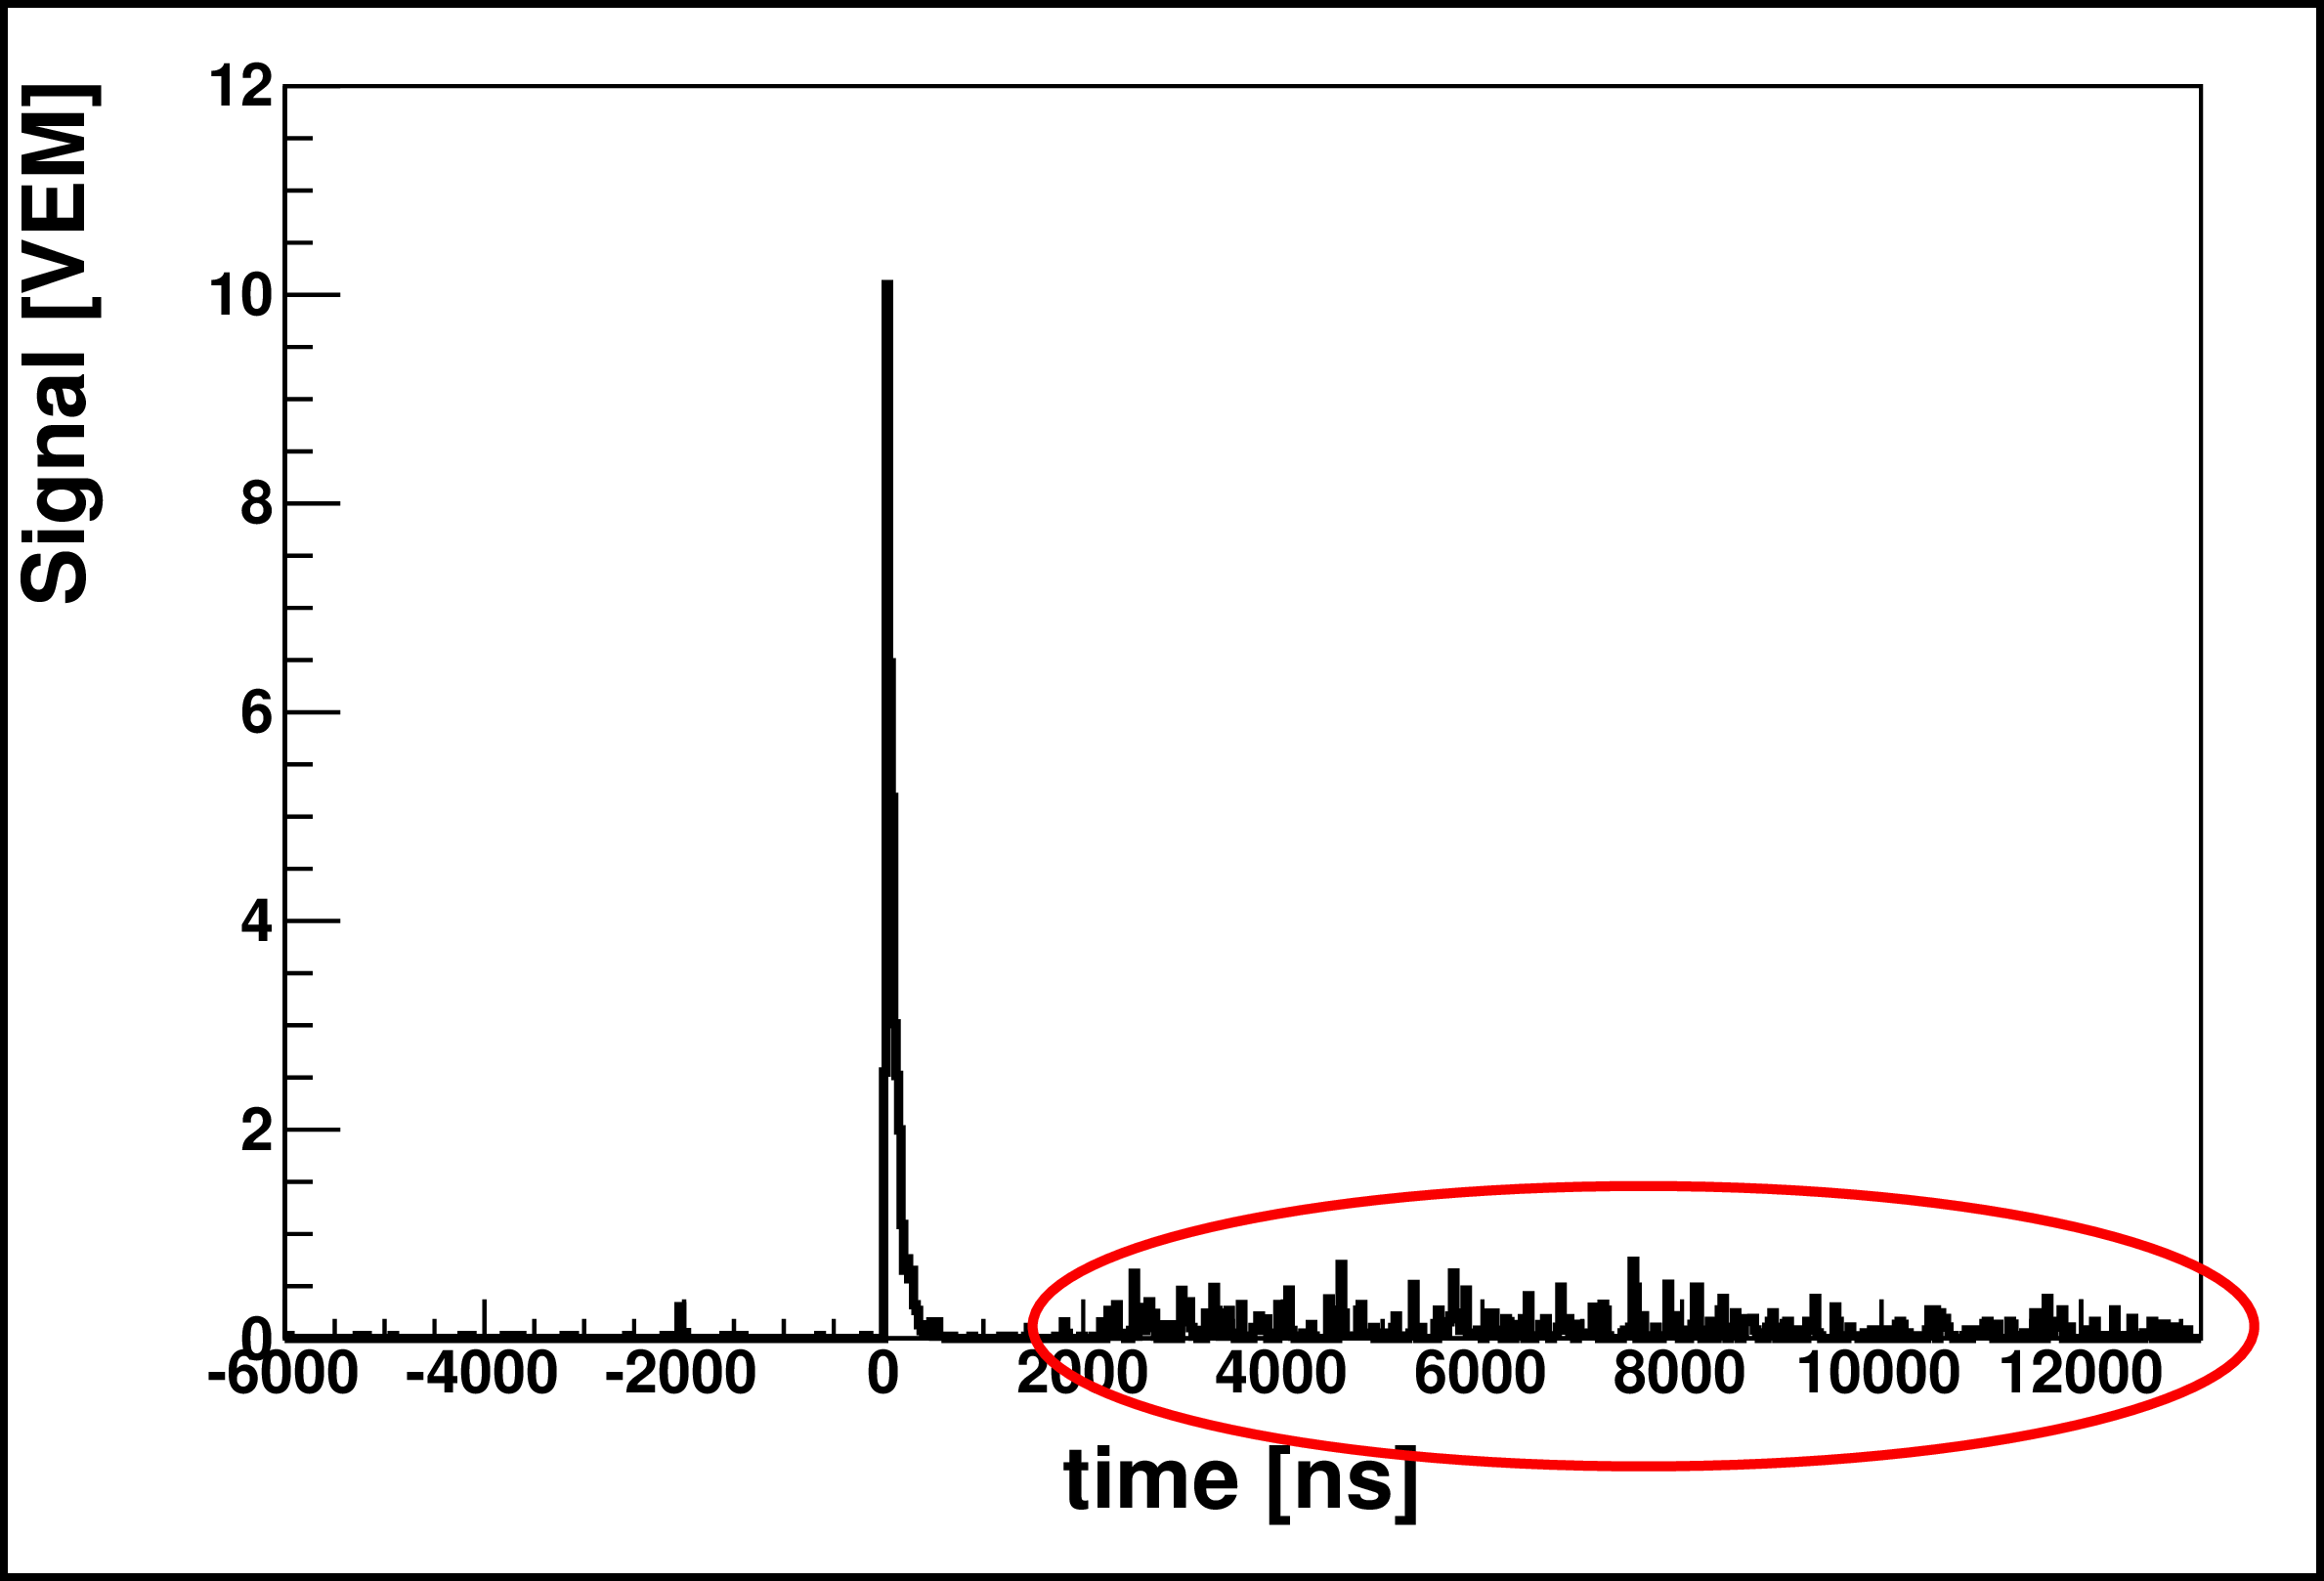
\includegraphics[width=0.48\textwidth]{fig/seleccionAuger/pmt2_border}\hspace*{2mm}
	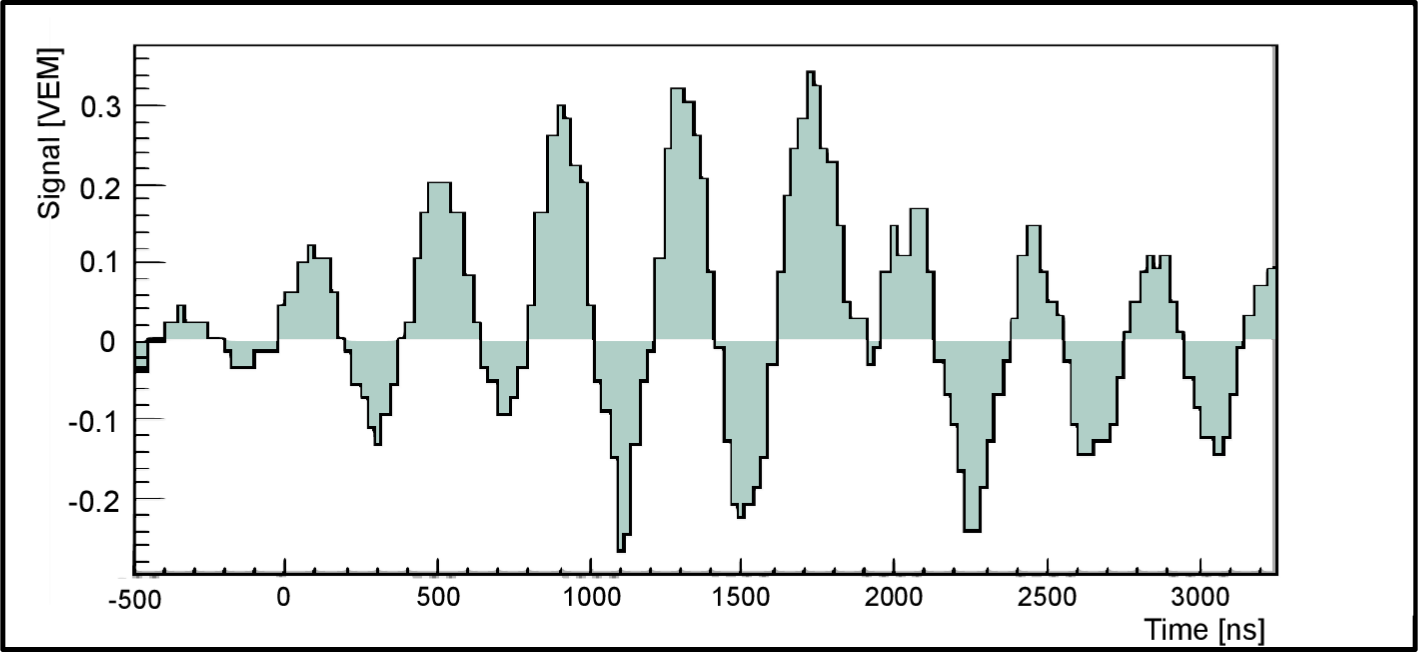
\includegraphics[width=0.48\textwidth]{fig/seleccionAuger/lighting}}
	\onslide<2>\centerline{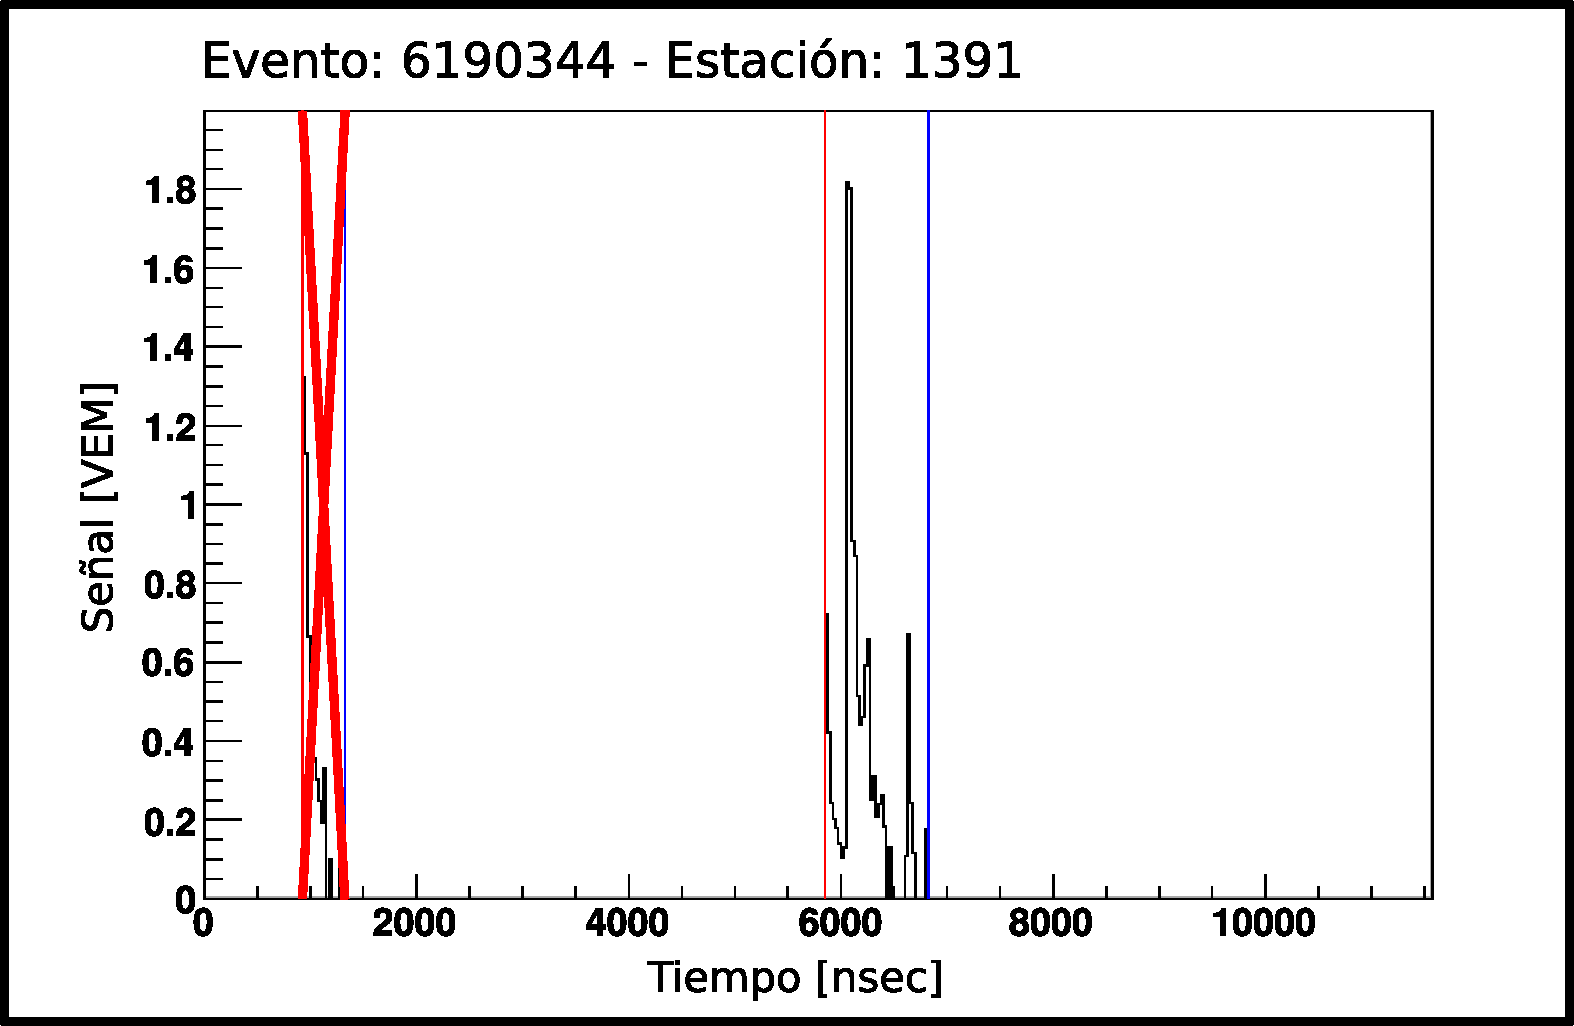
\includegraphics[height=0.35\textwidth]{fig/seleccionAuger/badStartTime_2}}
	\onslide<3>\centerline{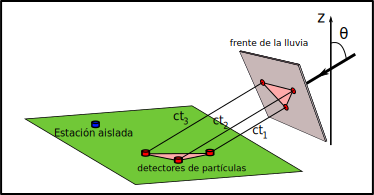
\includegraphics[height=0.35\textwidth]{fig/seleccionAuger/geome2}}
	\end{overprint}
	\end{exampleblock}
\end{frame}

\begin{frame}
 \frametitle{Selecci\'on de lluvias j\'ovenes}
 \begin{block}{Discriminante de Fisher}
 \centering
  \pgfimage[width=0.85\textwidth]{fig/seleccionAuger/ideaFisher}
 \end{block}
\end{frame}

\begin{frame}{Eficiencias DG}
	\begin{block}{Disparo com funci\'on de la prifundidad}
		\begin{center}
		\pgfimage[width=0.75\textwidth]{fig/exposicionAuger/eff_10EeV_85}
		\end{center}
	\end{block}
\end{frame}

\begin{frame}{Eficiencias DG}
	\begin{block}{Disparo com funci\'on de la energ\'ia}
		\begin{center}
		\pgfimage[width=0.75\textwidth]{fig/exposicionAuger/eff_varios_85}
		\end{center}
	\end{block}
\end{frame}

\begin{frame}{Eficiencias DG}
\footnotesize
	\begin{block}{Disparo com funci\'on del \'angulo cenital}
		\begin{center}
		\pgfimage[width=0.4\textwidth]{fig/exposicionAuger/eff_1EeV_80}\hspace{3mm}
		\pgfimage[width=0.4\textwidth]{fig/exposicionAuger/eff_1EeV_85}
		\end{center}
	\end{block}
% \end{frame}
% 
% \begin{frame}{Eficiencias DG}
	\begin{block}{Disparo com funci\'on del canal de interaccion}
		\begin{center}
		\pgfimage[width=0.4\textwidth]{fig/exposicionAuger/eff_CCvsNC_85}\hspace{3mm}
		\pgfimage[width=0.4\textwidth]{fig/exposicionAuger/eff_tau_1EeV_85}
		\end{center}
	\end{block}
\end{frame}

\begin{frame}{Eficiencias ES}
	\begin{block}{Disparo com funci\'on de la altura de decaimiento}
		\begin{center}
		\pgfimage[width=0.75\textwidth]{fig/exposicionAuger/eff_18_8931_forThesis}
		\end{center}
	\end{block}
\end{frame}

\begin{frame}{Eficiencias ES}
	\begin{block}{Disparo com funci\'on de la energ\'ia}
		\begin{center}
		\pgfimage[width=0.75\textwidth]{fig/exposicionAuger/eff_multEnergy_forThesis}
		\end{center}
	\end{block}
\end{frame}

\begin{frame}{Eficiencias ES}
\footnotesize
	\begin{block}{Disparo com funci\'on del \'angulo cenital}
		\begin{center}
		\pgfimage[width=0.48\textwidth]{fig/exposicionAuger/eff_multiTheta_forThesis}
		\hspace{1mm}
		\pgfimage[width=0.48\textwidth]{fig/exposicionAuger/eff_multTheta_h10_forThesis}
		\end{center}
	\end{block}
	\begin{block}{Definicion de la variable $h_{10}$}
		\begin{center}
		\pgfimage[width=0.45\textwidth]{fig/exposicionAuger/hc_def.pdf}
		\end{center}
	\end{block}
\end{frame}

\begin{frame}{Integraci\'on de las eficiencias}
	\begin{block}{M\'etodo de calculo}
	\begin{enumerate}[<uncover@+-|alert@+>]
	 \item Elegir una configuraci\'on representativa cada 3 dias.
	 \item Lanzar las lluvias sobre tal configuraci\'on y recalcular los criterios de disparo.
	 
	 \begin{center}  
		\visible<2->{\pgfimage[width=0.45\textwidth]{fig/exposicionAuger/aperturaReal}}
	 \end{center}
	 \item Calcular la integral como: $\sum_{t_i} {\cal A}_{circ} \times \frac{\#_{sel}}{\#_{sim}} \times \Delta T_i$
	\end{enumerate}

	\end{block}
\end{frame}

\begin{frame}{Integraci\'on temporal y en superficie}
	\begin{block}{M\'etodo de calculo}
		\begin{center}
		\pgfimage[width=0.6\textwidth]{fig/exposicionAuger/aperturaReal}
		\end{center}
	\end{block}
\end{frame}

\begin{frame}{Integraci\'on temporal y en superficie}
	\begin{block}{Selecci\'on de la configuraci\'on del detector}
		\begin{center}
		\pgfimage[width=0.75\textwidth]{fig/exposicionAuger/t2FilePlot}
		\end{center}
	\end{block}
\end{frame}


\begin{frame}{Integraci\'on temporal y en superficie}
	\begin{block}{Envejecimiento de detector}
		\begin{center}
		\pgfimage[width=0.9\textwidth]{fig/exposicionAuger/timeEvolution_1}<1>
		\pgfimage[width=0.9\textwidth]{fig/exposicionAuger/timeEvolution_2}<2>
		\pgfimage[width=0.9\textwidth]{fig/exposicionAuger/timeEvolution_3}<3>
		\pgfimage[width=0.9\textwidth]{fig/exposicionAuger/fractionEvolution}<4>
		\end{center}
	\end{block}
\end{frame}


\begin{frame}{Integraci\'on temporal y en superficie}
	\begin{block}{Envejecimiento de detector}
		\begin{center}
		\pgfimage[width=0.55\textwidth]{fig/exposicionAuger/timedecay_vs_reflect_absorp_2}
		\end{center}
	\end{block}
	\begin{block}{Envejecimiento de detector}<2>
		\begin{center}
		\renewcommand{\arraystretch}{1.4}
		\footnotesize
		\begin{tabular}{|l|ccc|c|}
					\hline
					Período       & tyRef & wAbs & LDT        &    Pérdida de exposición \\
					\hline
					$2004 - 2008$ & 0.94  & 100  & $\sim63$ns &    $--$ \\
					$2009 - 2010$ & 0.94  & 80   & $\sim60$ns &    $-15.2\%$\\
					$2011 - 2013$ & 0.93  & 100  & $\sim57$ns &    $-17.5\%$\\
					\hline
		\end{tabular}
		\end{center}
	\end{block}
\end{frame}

\begin{frame}{Exposici\'on combinada}
	\begin{block}{Obtenci\'on de la exposicion total}
		\begin{center}
			\begin{displaymath}\renewcommand{\arraystretch}{2}
			\begin{array}{rcl}
			N_{esp}& =& N_{esp}^{DGL}+N_{esp}^{DGH}+N_{esp}^{ES} \\ 
			& = & \int\limits_{E_\nu}\Phi(E_\nu)~({\cal E}^{DGL}+{\cal E}^{DGH}+{\cal E}^{ES})(E_\nu)~dE_\nu\\
			& \equiv & \int\limits_{E_\nu}\Phi(E_\nu)~{\cal E}(E_\nu)~dE_\nu
			\end{array}
			\end{displaymath}
		\end{center}
	\end{block}
	
	\begin{alertblock}{}
	\centering
% 		\begin{center}
			\begin{displaymath}
			{\cal E}(E_\nu) = {\cal E}^{DGL}+{\cal E}^{DGH}+{\cal E}^{ES}
			\end{displaymath}
% 		\end{center}
	\end{alertblock}
	
	\begin{exampleblock}{}
		\begin{center}
			\textbf{La exposici\'on combinada es la suma de las individuales}
		\end{center}
	\end{exampleblock}
\end{frame}

\begin{frame}{Exposici\'on combinada}
\framesubtitle{Escenario $\Phi\propto E^{-2}$}
	\begin{block}{Distribuci\'on de la exposici\'on}
		\begin{center}
		\begin{tabular}{|c|c|c|c|c|}
			\hline
			\diagbox{Lluvia}{Criterio} & ES & DGH & DGL  & Total\\ \hline
			ES     &    \alert<2>{0.80}& \alert<2>{0.04} & $<0.001$ & \alert<1>{0.84} \\ \hline
			DGH    &    \alert<3>{0.03}       &    \alert<3>{0.11}       &     $<0.001$ & \alert<1>{0.14} \\ \hline
			DGL    &    $<0.001$   &    $<0.001$   &     0.02     & \alert<1>{0.02} \\
			\hline
		\end{tabular}
		\end{center}
	\end{block}
	\begin{exampleblock}{Matriz de clasificaci\'on}<uncover@4->
		\begin{center}
		\begin{tabular}{|c|c|c|c|c|c|}
			\hline
			\diagbox{Lluvia}{Criterio} & ES $\wedge$ DGH &  ES    &  DGH   &  DGL      \\ \hline
			ES       & \alert<5>{0.90} &  \alert<6>{0.86}  &  \alert<7>{0.48}  &  \alert<8>{0.00}     \\ \hline
			DGH      & \alert<5>{0.10} &  \alert<6>{0.14}  &  \alert<7>{0.52}  &  \alert<8>{0.03}     \\ \hline
			DGL      & \alert<5>{0.00} &  \alert<6>{0.00}  &  \alert<7>{0.00}  &  \alert<8>{0.97}     \\ \hline\hline
			Probabilidad & \alert<9>{0.69} &  \alert<9>{0.20}  &  \alert<9>{0.09}  &  \alert<9>{0.02}     \\
			\hline
		\end{tabular}
		\end{center}
	\end{exampleblock}
\end{frame}

% \begin{frame}{Exposici\'on combinada}
% 	\begin{block}{Distribuci\'on de la exposici\'on}
% 		\begin{center}
% 		\begin{tabular}{|c|c|c|c|c|}
% 			\hline
% 			\diagbox{Lluvia}{Criterio} & ES & DGH & DGL  & Total\\ \hline
% 			ES     &    0.80       &    0.04       &     $<0.001$ & 0.84 \\ \hline
% 			DGH    &    0.03       &    0.11       &     $<0.001$ & 0.14 \\ \hline
% 			DGL    &    $<0.001$   &    $<0.001$   &     0.02     & 0.02 \\
% 			\hline
% 		\end{tabular}
% 		\end{center}
% 	\end{block}
% 	\begin{alertblock}{Matriz de clasificaci\'on}<uncover@2>
% 		\begin{center}
% 		\begin{tabular}{|c|c|c|c|c|c|}
% 			\hline
% 			\diagbox{Lluvia}{Criterio} & ES $\wedge$ DGH &  ES    &  DGH   &  DGL      \\ \hline
% 			ES                         & 0.90            &  0.86  &  0.48  &  0.00     \\ \hline
% 			DGH                        & 0.10            &  0.14  &  0.52  &  0.03     \\ \hline
% 			DGL                        & 0.00            &  0.00  &  0.00  &  0.97     \\ \hline\hline
% 			Probabilidad               & 0.69            &  0.20  &  0.09  &  0.02     \\
% 			\hline
% 		\end{tabular}
% 		\end{center}
% 	\end{alertblock}
% \end{frame}

\begin{frame}{Errores sistem\'aticos}
	\begin{alertblock}{Bines representativos en ES}
		\begin{center}
			\pgfimage[width=0.75\textwidth]{fig/exposicionAuger/importantBins_oldWeights}
		\end{center}
	\end{alertblock}
	\begin{block}{Resultado}
		\begin{center}
			Se recalculo la exposici\'on sobre los bines que m\'as contribuyen a la exposici\'on.
		\end{center}
	\end{block}
\end{frame}

\begin{frame}{Errores sistem\'aticos}
	\begin{block}{}
		\begin{center}
			\pgfimage[width=0.45\textwidth]{fig/exposicionAuger/nu_xsection_models}\hspace{2mm}
			\pgfimage[width=0.45\textwidth]{fig/exposicionAuger/tau_E_loss_models}
		\end{center}
	\end{block}
	\begin{exampleblock}{}
		\begin{center}
			\begin{tabular}{|l|l|l|}
			\hline
			\textbf{Modelo}      & Secci\'on eficaz& P\'erdida de energ\'ia del $\tau$ \\ 
			\hline
			Referencia &    Sarkar     & ALLM\\ 
			%
			Pesimista &  ASW &     BB\\ 
			%
			Optimista &   Armesto Sat. $\lambda=0.4$&  ASW\\
			\hline 
			\end{tabular}  
		\end{center}
	\end{exampleblock}
\end{frame}

\begin{frame}{Errores sistem\'aticos}
	\begin{block}{Cambio en las probabilidades}
		\begin{center}
			\pgfimage[width=0.75\textwidth]{fig/exposicionAuger/pdfSyst}
		\end{center}
	\end{block}
	\begin{exampleblock}{Resultado}
		\begin{center}
			Cambian la probabilidad de emerger y el espectro de energ\'ia.
		\end{center}
	\end{exampleblock}
\end{frame}


\begin{frame}{Unblinding DGL}
	\begin{center}
	\pgfimage[width=0.75\textwidth]{fig/resultadosAuger/DGL_Unblinding_Thesis}
	\end{center}
	\begin{block}{}
	\centering {\Large \color{red}\bf 0 candidatos}
	\end{block}
\end{frame}


\begin{frame}{Emisi\'on de radio en lluvias atmosf\'ericas}
\framesubtitle{Origen}
\footnotesize
	
	\begin{block}{Part\'icula que se desplaza en l\'inea recta a velocidad constante}
		\begin{center}
		\pgfimage[width=0.5\textwidth]{fig/EASRadio/trackSch}
		\end{center}
	\end{block}
	
	\begin{block}{Aproximaci\'on ZHS}
		\begin{center}
		\pgfimage[width=0.5\textwidth]{fig/EASRadio/zhs_pulse}
		\end{center}
	\end{block}
\end{frame}

\begin{frame}{Emisi\'on de radio en lluvias atmosf\'ericas}
\framesubtitle{Huella y estructura temporal}
\footnotesize
	\begin{block}{Cono Cherenkov}
		\begin{overprint}
		\onslide<1>\centerline{\pgfimage[width=0.9\textwidth]{fig/EASRadio/cherEmmision}}
		\onslide<2>\centerline{\pgfimage[width=0.9\textwidth]{fig/EASRadio/cono}}
		\onslide<3>\centerline{\pgfimage[width=0.9\textwidth]{fig/EASRadio/chConeSch}}
		\end{overprint}
	\end{block}
	\begin{alertblock}{}<3>
	\centering
	\alert<3>{\textbf{Anillo Cherenkov}}
	\end{alertblock}
\end{frame}

\begin{frame}{Modelo de juguete}
\footnotesize
	\begin{exampleblock}{Esquema}
		\begin{center}
		\pgfimage[width=0.85\textwidth]{fig/modeloRadio/timeDelaySchema}
		\end{center}
	\end{exampleblock}
	\begin{block}{Resultado}<2>
		\begin{center}
		\visible<2>{
		\pgfimage[height=0.25\textwidth]{fig/modeloRadio/timeDelay_pd} \hspace*{0mm}
		\pgfimage[height=0.25\textwidth]{fig/modeloRadio/legend.pdf} \hspace*{0mm}
		\pgfimage[height=0.25\textwidth]{fig/modeloRadio/timeDelay_spa} \hspace*{0mm}
		}
		\end{center}
	\end{block}
\end{frame}

\begin{frame}{Ubicaci\'on del detector}
\footnotesize
	\begin{block}{Posibles ubicaciones}
		\begin{center}\scriptsize
		\begin{tabular}{LLLL}
		\toprule
		Experimento (Sitio) & Declinaci\'on (+E,-W) & Inclinaci\'on (+D,-U)& Intensidad [Gauss] \\
		\midrule
		Auger AERA (Malarg\"ue Argentina) 
% 		& $35^\circ12$'${\rm S} $ $69^\circ18$'${\rm W}$
		& $(1.68\pm0.37)^\circ$ & $(-36.3\pm0.22)^\circ$ & $0.2392\pm0.0015$ \\ \midrule
		\alert<2>{Tunka Rex  (Tunka Valley Rusia)}
% 		& $51^\circ48$'${\rm N}$ $103^\circ04$'${\rm E}$
		& \alert<2>{$(-2.82\pm0.37)^\circ$} & \alert<2>{$(-71.2\pm0.22)^\circ$} & \alert<2>{$0.6037\pm0.0015$} \\ \midrule
		Trend  (Tian shan China) 
% 		& $40^\circ32$'${\rm N}$ $78^\circ25$'${\rm E}$
		& $(3.76\pm0.37)^\circ$ & $(60.0\pm0.22)^\circ$ & $0.5391\pm0.0015$ \\
		\bottomrule
		\end{tabular}
		\end{center}
	\end{block}
	\begin{exampleblock}{Caracter\'isticas deseables}
	\begin{itemize}
	 \item Verticalidad
	 \item Intensidad 
	\end{itemize}
	\end{exampleblock}

\end{frame}

\begin{frame}{Representaci\'on del detector}
\footnotesize
	\begin{block}{Esquema del detector}
		\begin{center}
		\pgfimage[width=0.85\textwidth]{fig/simulacionRadio/antennaSch.pdf}
		\end{center}
	\end{block}
% 	\begin{alertblock}{Antena sobre el cono Cherenkov}
% 	\begin{center}
% 		\pgfimage[width=0.48\textwidth]{fig/simulacionRadio/antennaSignal}\hspace*{2mm}
% 		\pgfimage[width=0.48\textwidth]{fig/simulacionRadio/antennaFilt}
% 	\end{center}
% 	\end{alertblock}
\end{frame}

\begin{frame}{Disparo local - Fuentes de ruido}
\footnotesize
	\begin{exampleblock}{Fuentes}
	\begin{itemize}
	 \item Ionosf\'erico
	 \item Proveniente de la ciudad
	 \item Gal\'actico
	 \item Intr\'inseco
	\end{itemize}
	\end{exampleblock}
	\begin{block}{Intensidad}
		\begin{center}
		\pgfimage[width=0.5\textwidth]{fig/simulacionRadio/allanNoise.pdf}
		\end{center}
	\end{block}
	\vspace*{-1cm}
	\visible<2>{
		\begin{alertblock}{}
			\begin{center}
			\textbf{Nivel de disparo local entre \cant{\bm{40}}{\bm{\mu V/m}} y \cant{\bm{250}}{\bm{\mu V/m}}}
			\end{center}
		\end{alertblock}
		}
\end{frame}

\begin{frame}{Caracterizaci\'on}
\footnotesize
	
	\begin{overprint}
	 \onslide<1>
	 \begin{block}{Polarizaci\'on}
	 \begin{center}
		\pgfimage[width=0.85\textwidth]{fig/caracterizacionRadio/malField} 
		\end{center}
	\end{block}
	 \onslide<2>
	 \begin{block}{Polarizaci\'on}
		\begin{center}
		\pgfimage[width=0.48\textwidth]{fig/caracterizacionRadio/foorPrint_ZWv1.22_ntuples_v1.21_ChTest_phi_90_18_89.5_90_25_1238_E0x_u} $\ \ $
		\pgfimage[width=0.48\textwidth]{fig/caracterizacionRadio/foorPrint_ZWv1.22_ntuples_v1.21_ChTest_phi_90_18_89.5_90_25_1238_E0z_u} \\
		\vspace*{2mm}
		\pgfimage[width=0.48\textwidth]{fig/caracterizacionRadio/foorPrint_ZWv1.22_ntuples_v1.21_ChTest_phi_90_18_89.5_90_25_1238_E0y_u} $\ \ $
		\pgfimage[width=0.48\textwidth]{fig/caracterizacionRadio/phiDist_Test_18_89.5_90_25_1238}
		\end{center}
	\end{block}
	\end{overprint}

	
\end{frame}

\begin{frame}{C\'alculo de la eficiencia}
\footnotesize
	\begin{block}{Se lanz\'o cada lluvia 1000 veces sobre la celda primitiva}
	\centering
		\pgfimage[width=0.48\textwidth]{fig/resultadosRadio/17.00_89.90_00.00_00025_01238_1000_1000_90_re}\hspace*{2mm}
		\pgfimage[width=0.48\textwidth]{fig/resultadosRadio/17.00_89.90_00.00_00025_01238_1500_1500_60_re} \\ \vspace*{2mm}
		\pgfimage[width=0.48\textwidth]{fig/resultadosRadio/17.00_89.90_00.00_00025_01238_500_4000_90_de}\hspace*{2mm}
		\pgfimage[width=0.48\textwidth]{fig/resultadosRadio/17.00_89.90_00.00_00025_01238_750_750_60_hc}
	\end{block}
% 	\begin{block}{}
% 		\begin{center}
% 		
% 		\end{center}
% 	\end{block}
\end{frame}

\begin{frame}{Desempe\~no: Radio vs. Auger}
\footnotesize
	\begin{block}{Tama\~no dle detector}
	\centering
		\pgfimage[width=0.85\textwidth]{fig/resultadosRadio/area/Area_de}
	\end{block}
	
% 	\begin{block}{}
% 		\begin{center}
% 		
% 		\end{center}
% 	\end{block}
\end{frame}

\begin{frame}{Desempe\~no - L = 500 ${\rm km}$}
	\begin{block}{Rate de eventos}
		\begin{center}
		\renewcommand{\arraystretch}{1.3}
		\footnotesize
		\begin{tabular}{lccc}
			\hline
			\multirow{2}{*}{Modelo} & \multicolumn{3}{c}{Topograf\'ia - \cant{L=500}{km}} \\
			&   Regular &   Panal de abeja &   Bordes densos \\
			\hline
			Cosmogénico - proton, FRII &    185.8 &            193   &           191.3 \\
			Cosmogénico - proton, Fermi-LAT &     140.3 &             146.0 &           144.8 \\
			Cosmogénico - proton, SFR &     42.1 &             43.8   &            43.4 \\
			Cosmogénico - H\'ibrido &  23.9 - 61.3 &   24.8 - 63.7 &  24.6 - 63.2 \\
			Cosmogénico - iron, FRII &     13.0   &        13.4 &            13.3 \\
			IceCube extrapolado $E^{-2}$ &      53.6 &         55.5   &            55   \\
			IceCube extrapolado \emph{Best fit} &    52.4 &  53.8  &   53.3 \\
			\hline
		\end{tabular}
		\end{center}
	\end{block}
\end{frame}

\begin{frame}{Detector ideal}
\footnotesize
		\begin{alertblock}{Caracter\'isticas:}
		 \centering
		 \textbf{100$\bm\%$ eficiente en el rango angular $\bm{90^\circ}$ - $\bm{92.5^\circ}$}
		\end{alertblock}

		\begin{block}{\scriptsize L\'imite diferencial: 90000 antennas - Trigger local 50${\rm \mu Vm}$ - L = 250 ${\rm km}$ - 500${\rm km}$}
			\begin{center}
			\pgfimage[width=0.9\textwidth]{fig/resultadosRadio/limits_future_v1_1_2.pdf}
			\end{center}
		\end{block}
\end{frame}